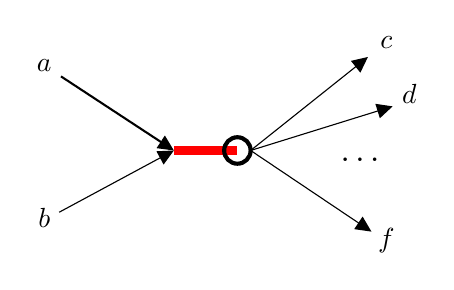
\begin{tikzpicture}[x=0.75pt,y=0.75pt,yscale=-0.85,xscale=0.85]
%uncomment if require: \path (0,140); %set diagram left start at 0, and has height of 140

%Straight Lines [id:da16249976297719293] 
\draw [line width=0.75]    (24.5,33) -- (86.83,73.9) ;
\draw [shift={(88.5,75)}, rotate = 213.27] [fill={rgb, 255:red, 0; green, 0; blue, 0 }  ][line width=0.75]  [draw opacity=0] (8.93,-4.29) -- (0,0) -- (8.93,4.29) -- cycle    ;

%Straight Lines [id:da772784293523332] 
\draw    (23.5,110) -- (86.74,75.95) ;
\draw [shift={(88.5,75)}, rotate = 511.7] [fill={rgb, 255:red, 0; green, 0; blue, 0 }  ][line width=0.75]  [draw opacity=0] (8.93,-4.29) -- (0,0) -- (8.93,4.29) -- cycle    ;

%Straight Lines [id:da9613918488192326] 
\draw [color={rgb, 255:red, 255; green, 0; blue, 0 }  ,draw opacity=1 ][line width=3]    (88.5,75) -- (124.5,75) ;


%Shape: Circle [id:dp6094178436022282] 
\draw  [line width=1.5]  (117,75) .. controls (117,70.86) and (120.36,67.5) .. (124.5,67.5) .. controls (128.64,67.5) and (132,70.86) .. (132,75) .. controls (132,79.14) and (128.64,82.5) .. (124.5,82.5) .. controls (120.36,82.5) and (117,79.14) .. (117,75) -- cycle ;
%Straight Lines [id:da9688539202688002] 
\draw    (132,75) -- (196.94,23.25) ;
\draw [shift={(198.5,22)}, rotate = 501.45] [fill={rgb, 255:red, 0; green, 0; blue, 0 }  ][line width=0.75]  [draw opacity=0] (8.93,-4.29) -- (0,0) -- (8.93,4.29) -- cycle    ;

%Straight Lines [id:da9340506100154327] 
\draw    (132,75) -- (210.59,50.59) ;
\draw [shift={(212.5,50)}, rotate = 522.75] [fill={rgb, 255:red, 0; green, 0; blue, 0 }  ][line width=0.75]  [draw opacity=0] (8.93,-4.29) -- (0,0) -- (8.93,4.29) -- cycle    ;

%Straight Lines [id:da7562683529308978] 
\draw    (132,75) -- (198.84,119.89) ;
\draw [shift={(200.5,121)}, rotate = 213.88] [fill={rgb, 255:red, 0; green, 0; blue, 0 }  ][line width=0.75]  [draw opacity=0] (8.93,-4.29) -- (0,0) -- (8.93,4.29) -- cycle    ;


% Text Node
\draw (15,27) node  [align=left] {$a$};
% Text Node
\draw (15,113) node  [align=left] {$b$};
% Text Node
\draw (209,14) node  [align=left] {$c$};
% Text Node
\draw (222,43) node  [align=left] {$d$};
% Text Node
\draw (209,126) node  [align=left] {$f$};
% Text Node
\draw (194,80) node [scale=1.2] [align=left] {$\dots$};


\end{tikzpicture}